\documentclass[12pt]{article}
\usepackage[utf8]{inputenc}
\usepackage{graphicx}
\usepackage[section]{placeins}

\title{Markov-Lokalisierung}
\author{Özgür Gümüslü}
\date{April 2021}

\begin{document}
\maketitle
\tableofcontents
\newpage

\section{Aufgabenstellung}
In dieser Hausübung ist es die Aufgabe die Wahrscheinlichste Position eines Roboters, welche sich in einem 1 dimensionalen Raum bewegt über die Markov basierte Lokalisierung zu bestimmen. Für genauere Angaben siehe Aufgabenblatt.

\section{Initialposition}
Die Initialposition des Roboters ist unbekannt, deshalb kann man von einer Gleichverteilung über der Map welche 50 Zellen lang ist rechnen.
$$bel(x_0) = \frac{1}{50} = \underline{0.02}$$

\begin{figure}[h]
    \centering
    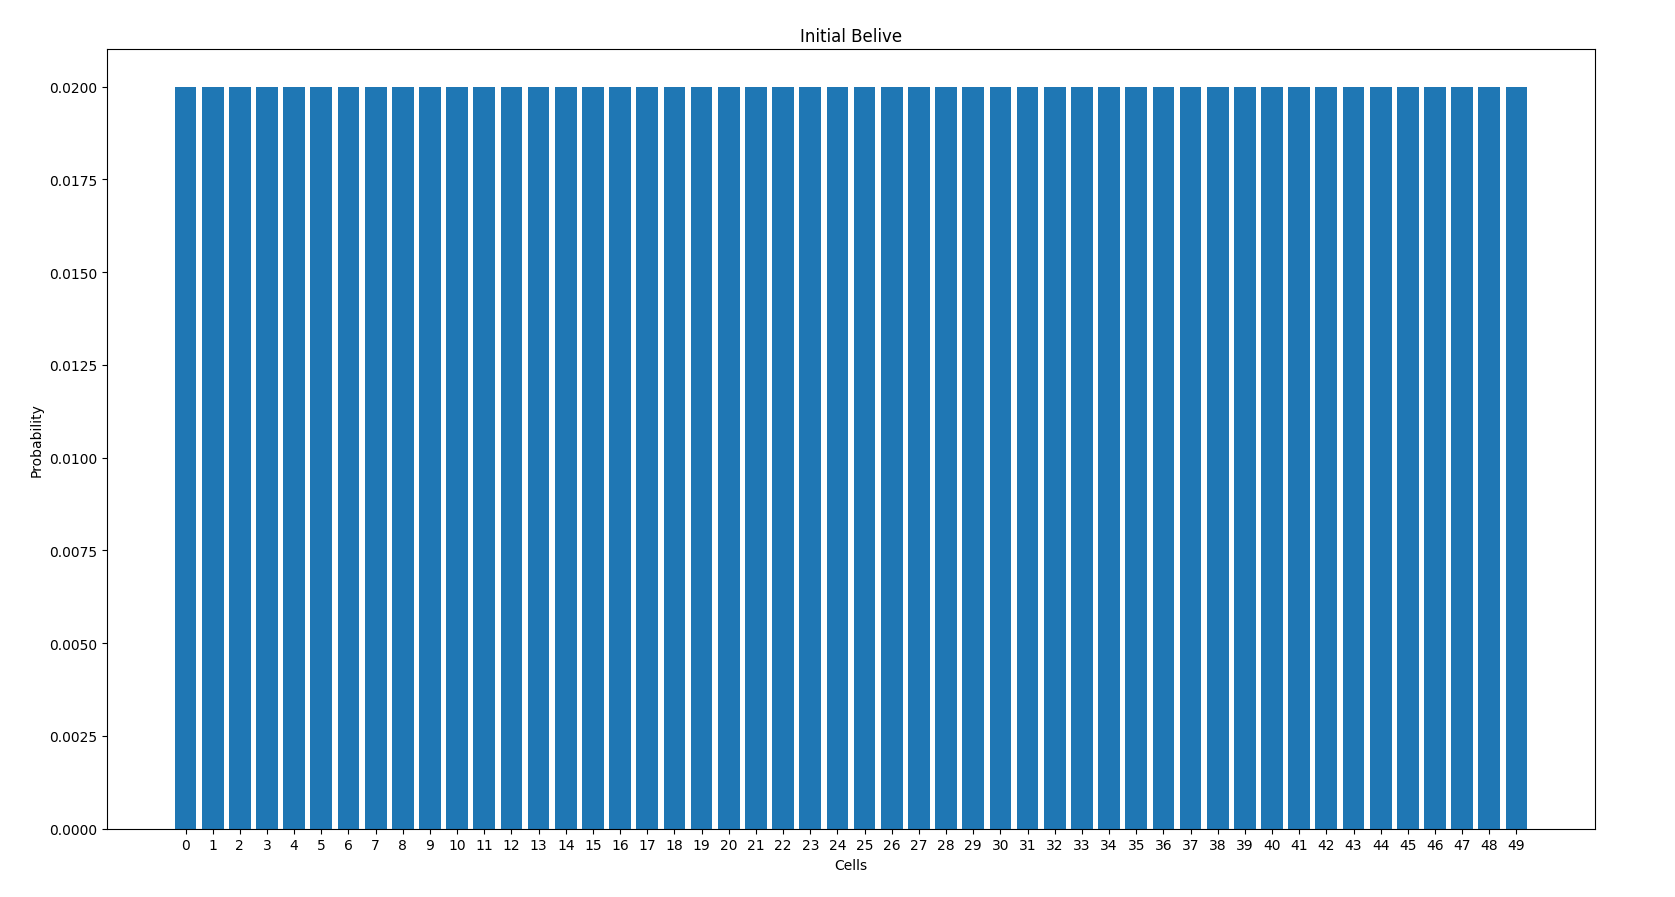
\includegraphics[width=1.3\textwidth]{img/bel(x0).png}
    \caption{Initiale Postion ist Gleichverteilt}
    \label{fig:Initiale Position}
\end{figure}

\section{Dokumentation zur Ermittlung der Position}
\subsection{Prediction Update}
Nach der Bestimmung des Startpostion wird versucht anhand des Bewegungsmodells die Roboterposition zu bestimmen. Dies wird mit Hilfe der Odometrie Daten berechnet (zb. Encoder). Die aktuelle Position wird wie folgt berechnet:
$$\overline{bel(x_t)} = \int p(x_t|u_t, x_{t-1})bel(x_{t-1})dx_{t-1}$$ im kontiniurlichem Bereich.
$$\overline{bel(x_t)} = \sum\limits_{x_{t-1}}p(x_t|u_t, x_{t-1})bel(x_{t-1})$$ im diskreten Bereich.\\

Wie man dem Algorithmus entnehmen kann berechnet sich der aktuelle 
believe ($\overline{bel(x_t)}$) durch die Wahrscheinlichkeit der aktuellen Position bedingt unter der aktuellen Messung der odometrischen Daten multipliziert mit dem exteroceptiven Daten der Sensoren (Posteriori Belive) des vorherigen Schrittes welche im Perception Update berechnet werden.
Hierbei wird das Theorem der totalen Wahrscheinlichkeit angewendet.

Im konkreten Beispiel wird über jede Zelle iteriert und die totale Wahrscheinlichkeit berechnet. Das Bewegungsmodell sagt folgendes aus:
Eine Vorwärtsbewegung liegt zwischen 3 und 7 Schritten mit entsprechen Wahrscheinlichkeiten:

\begin{itemize}
\item 3 Schritte  : 0.1
\item 4 Schritte : 0.2
\item 5 Schritte : 0.4
\item 6 Schritte : 0.2
\item 7 Schritte : 0.1
\end{itemize} 

In der Schleife wird nun für jede Zelle die Summe der Schritte mit den entsprechenden Wahrscheinlichkeiten aufsummiert. Somit erhalten wir eine Liste für $bel(x_t)$ mit den ensprechenden Wahrscheinlichkeiten für jede Zelle nach einer Bewegung.

$$\overline{bel(x_t)} = Gridmap[x_t-3] * p(3) + Gridmap[x_t-4] * p(4)+...+Gridmap[x_t-7] * p(7)$$

\subsection{Measurement Update} 
Hier geht es um die Korrektur des Prediction Updates. Die Daten von den odometrischen Daten werden hier mit den exteroceptiven Sensoren korrigiert. Hier kommt das Bayes Theorem zum tragen.
$$bel(x_t) = \eta\rho(z_t|x_t, M)\overline{bel(x_t)}$$

Der Algorithmus besagt dass die korrigierte Position($bel(x_t)$) sich mit der Wahrscheinlichkeit der Messdaten der Sensoren unter der Bedingung der aktuellen Position und den Landmarken(Karte) unter der multiplikation mit der berechneten Position aus dem Priori berechnen lässt. Dieses Ergebnis muss noch mit $\eta$ normalisiert werden welches nicht 0 sein darf.\\

Bevor die Posteriori Liste berechnet wurde, wurde eine Karte erstellt die, die entsprechenden Warscheinlichkeiten in der Mappe eingetragen hat(pMap).

Hier wurde an den Position an denen eine Säule steht für die Position die Wahrscheinlichkeit 0.5 eingetragen. Für eine Postion davor und danach wurde 0.25 eingetragen. Alle anderen Position wurde mit $10^{-5}$ berücksichtigt.

Nun wird wieder über jede Zelle iteriert und der Posterior noch nicht normalisiert berechnet:

$$bel(x_t) = pMap[x_t + sensormessung(pro Schritt)] * \overline{bel(x_t)}$$

Hier muss noch drauf geachtet werden, dass wenn die $x_t$ beim Überlauf wieder von vorne Anfängt. Zusätzlich sollte eine Messung die Distanz zur übernächste Säule liefern, darf dieser nicht in die Berechnung miteinfliessen.

Nachdem, dass über die ganze Map berechnet wurde werden die Wahrscheinlichkeiten aufsummiert um mit der Kehrwertbildung den Normalisierungsfaktor $\eta$ zu erhalten. Dieser wird dann mit der Liste multipliziert um den Posterior zu erhalten.
 

\section{Ermittelung des Messmodells}
Das Messmodell wird im wesentlichen im Punkt 3.2 erklärt.
Es sagt dabei die Wahrscheinlichkeit einer Position in der Wahrscheinlichkeitsbasierten Mappe (pMap) bei der aktuellen Position + Sensorwert.

$$pMap[x_t + sensormessung(pro Schritt)]$$

\section{Prior und Posterior Ergebnisse der einzelnen Schritte}
Hier werden die Prior und Posterior plots für die einzelnen Schritte 5, 10, 7, 2, 10 visualisiert.


\begin{figure}[h]
    \centering
    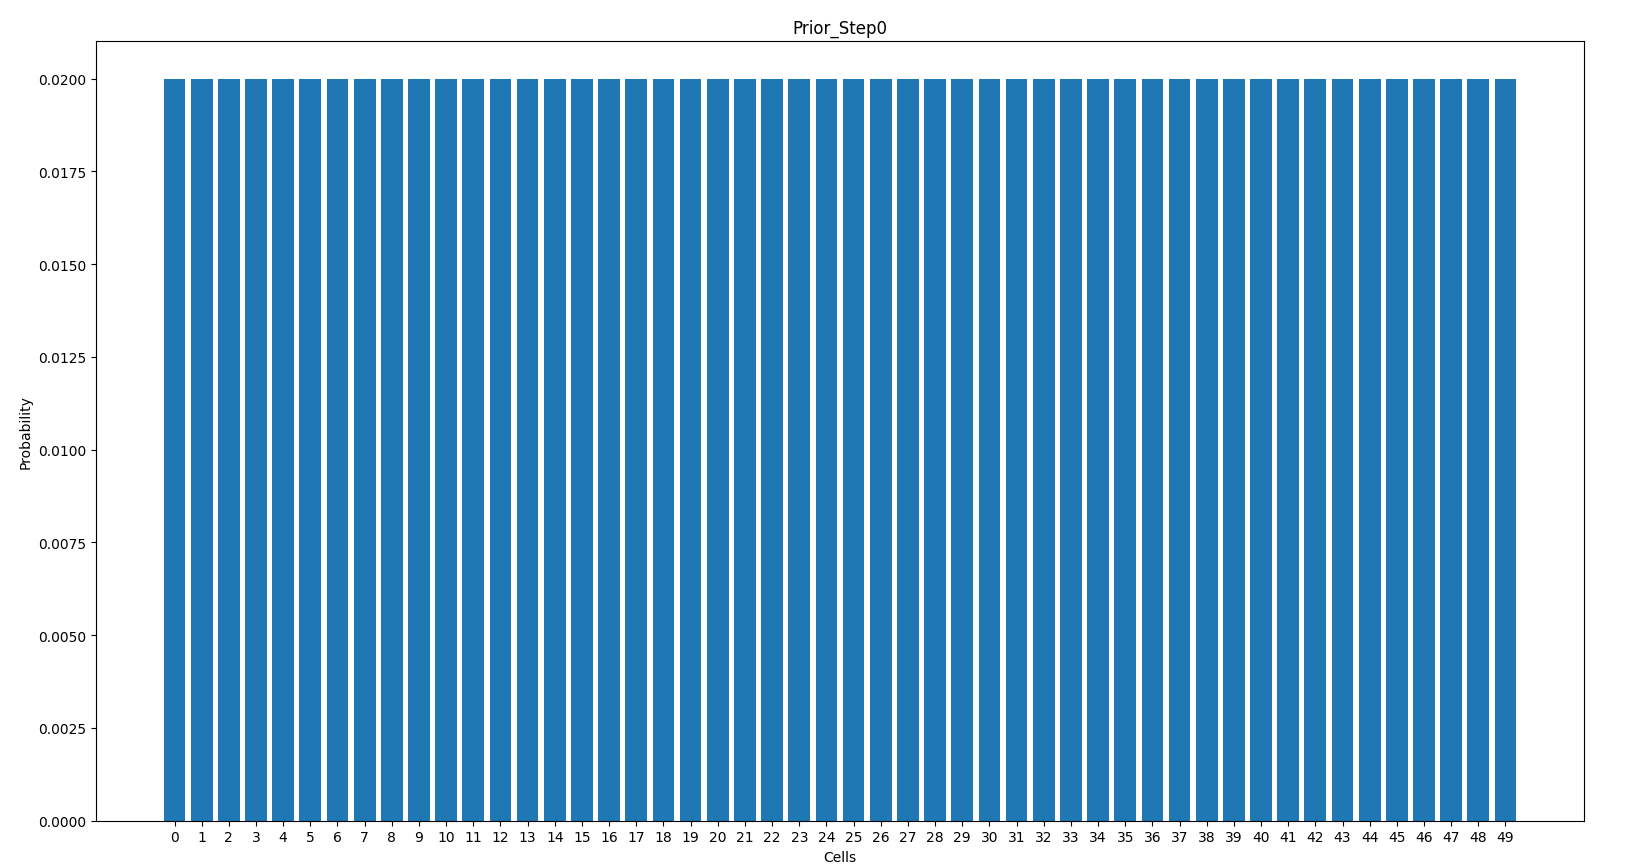
\includegraphics[width=1.3\textwidth]{img/prior_step_0.png}
    \caption{Prior Believe nach dem ersten Schritt=5}
    \label{fig:Prior Believe nach dem ersten Schritt=5}
\end{figure}

\begin{figure}[h]
    \centering
    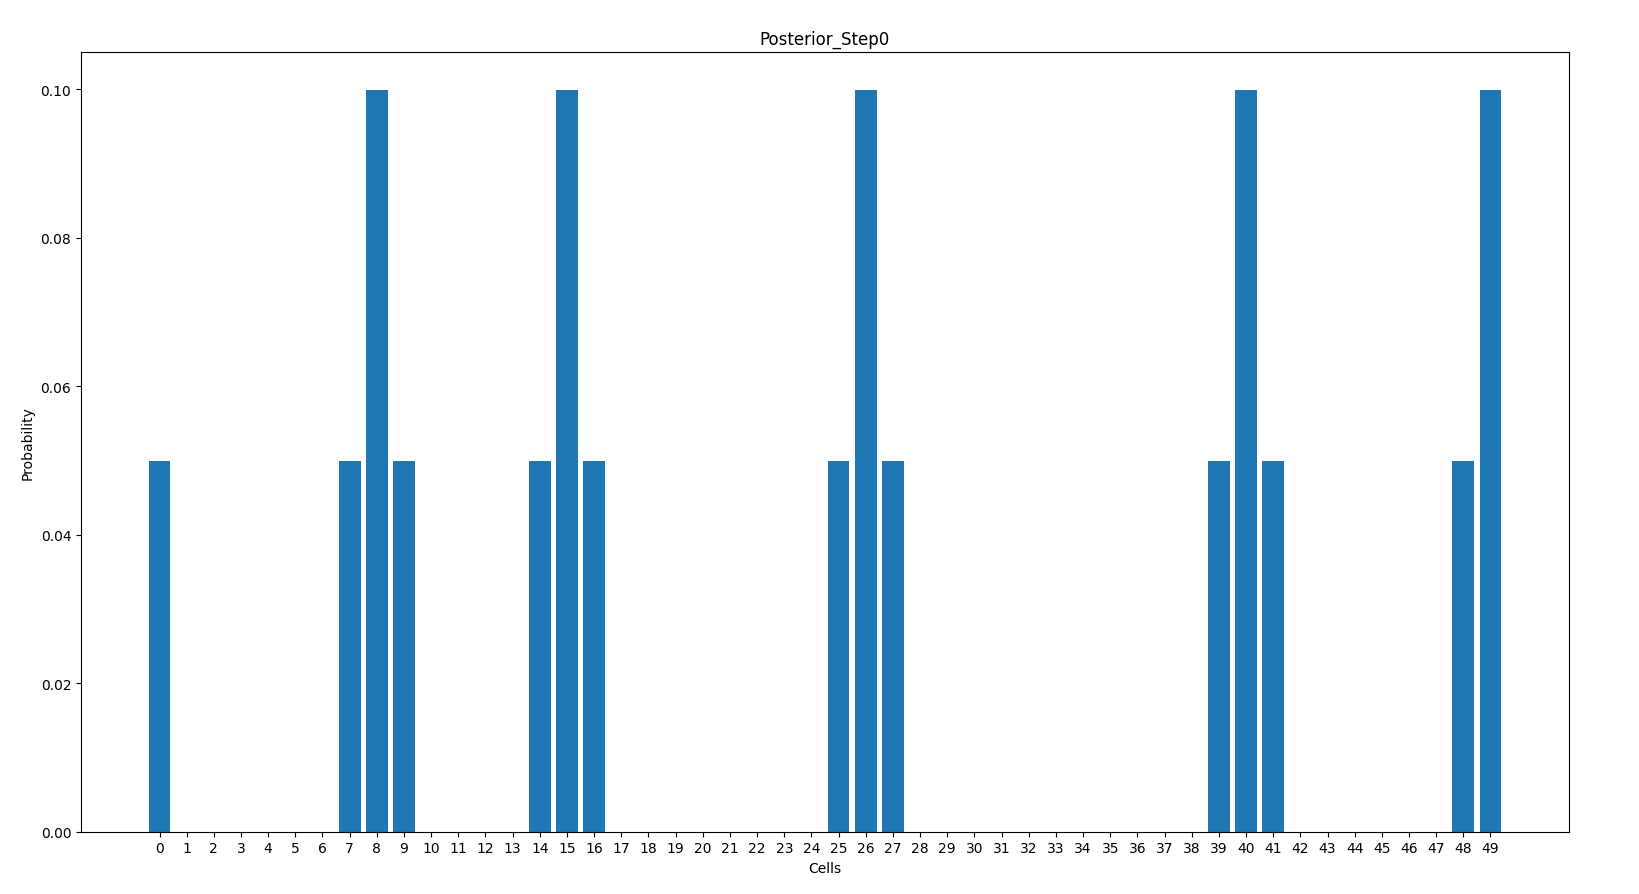
\includegraphics[width=1.3\textwidth]{img/posterior_step_0.png}
    \caption{Posterior Believe nach dem ersten Schritt=5}
    \label{fig:Posterior Believe nach dem ersten Schritt=5}
\end{figure}

\begin{figure}[h]
    \centering
    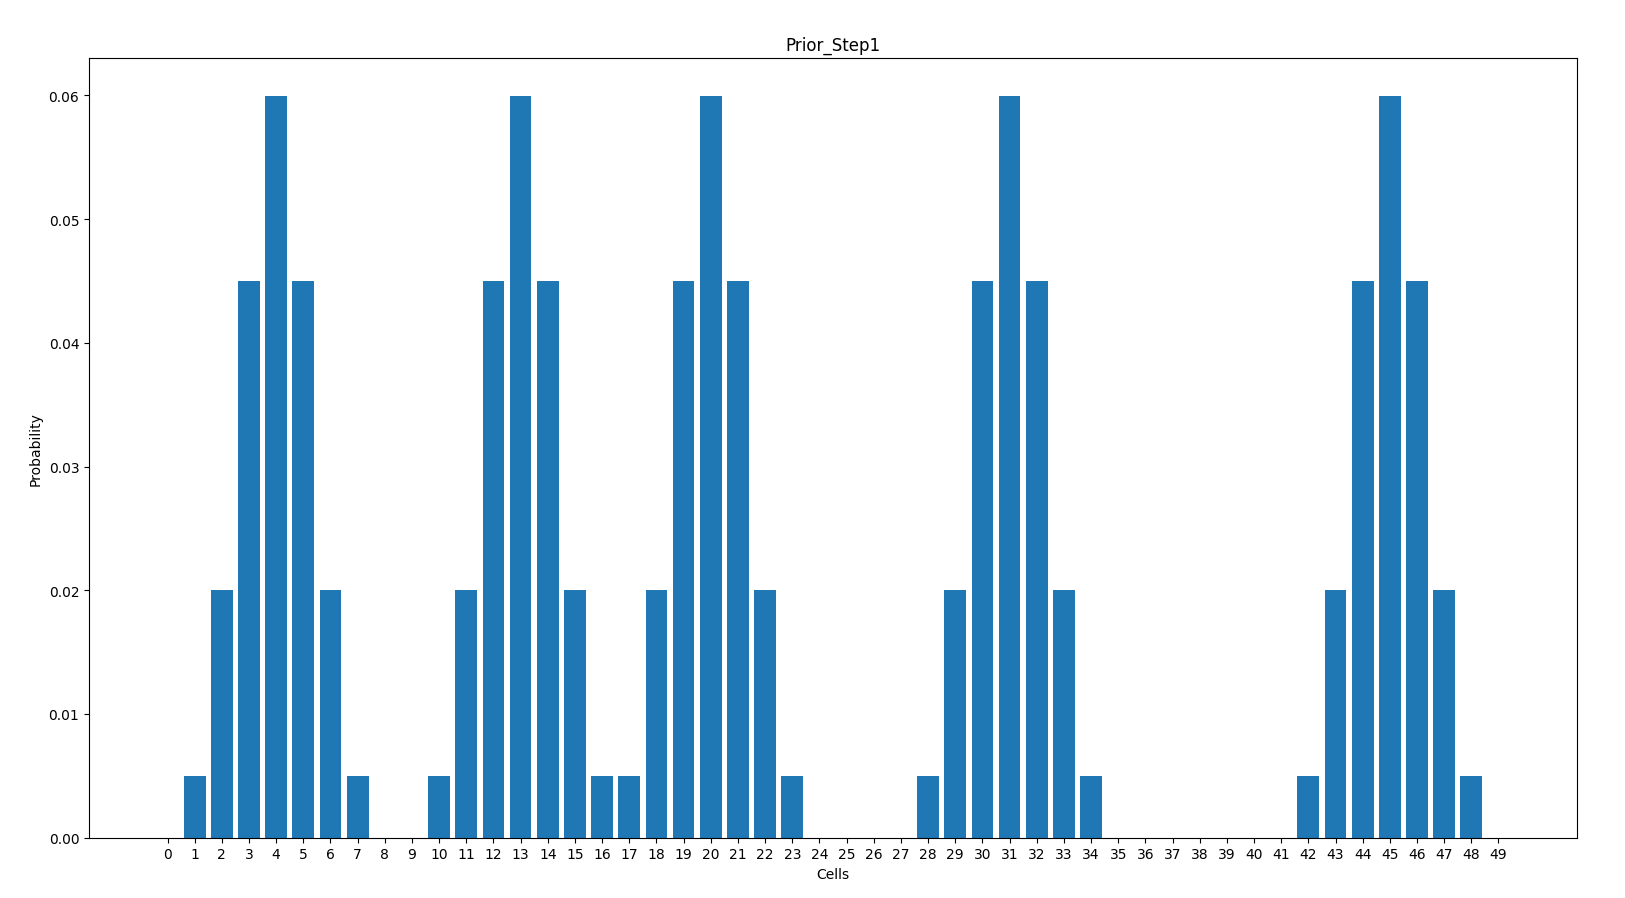
\includegraphics[width=1.3\textwidth]{img/prior_step_1.png}
    \caption{Prior Believe nach dem zweitem Schritt=10}
    \label{fig:Prior Believe nach dem zweitem Schritt=10}
\end{figure}

\begin{figure}[h]
    \centering
    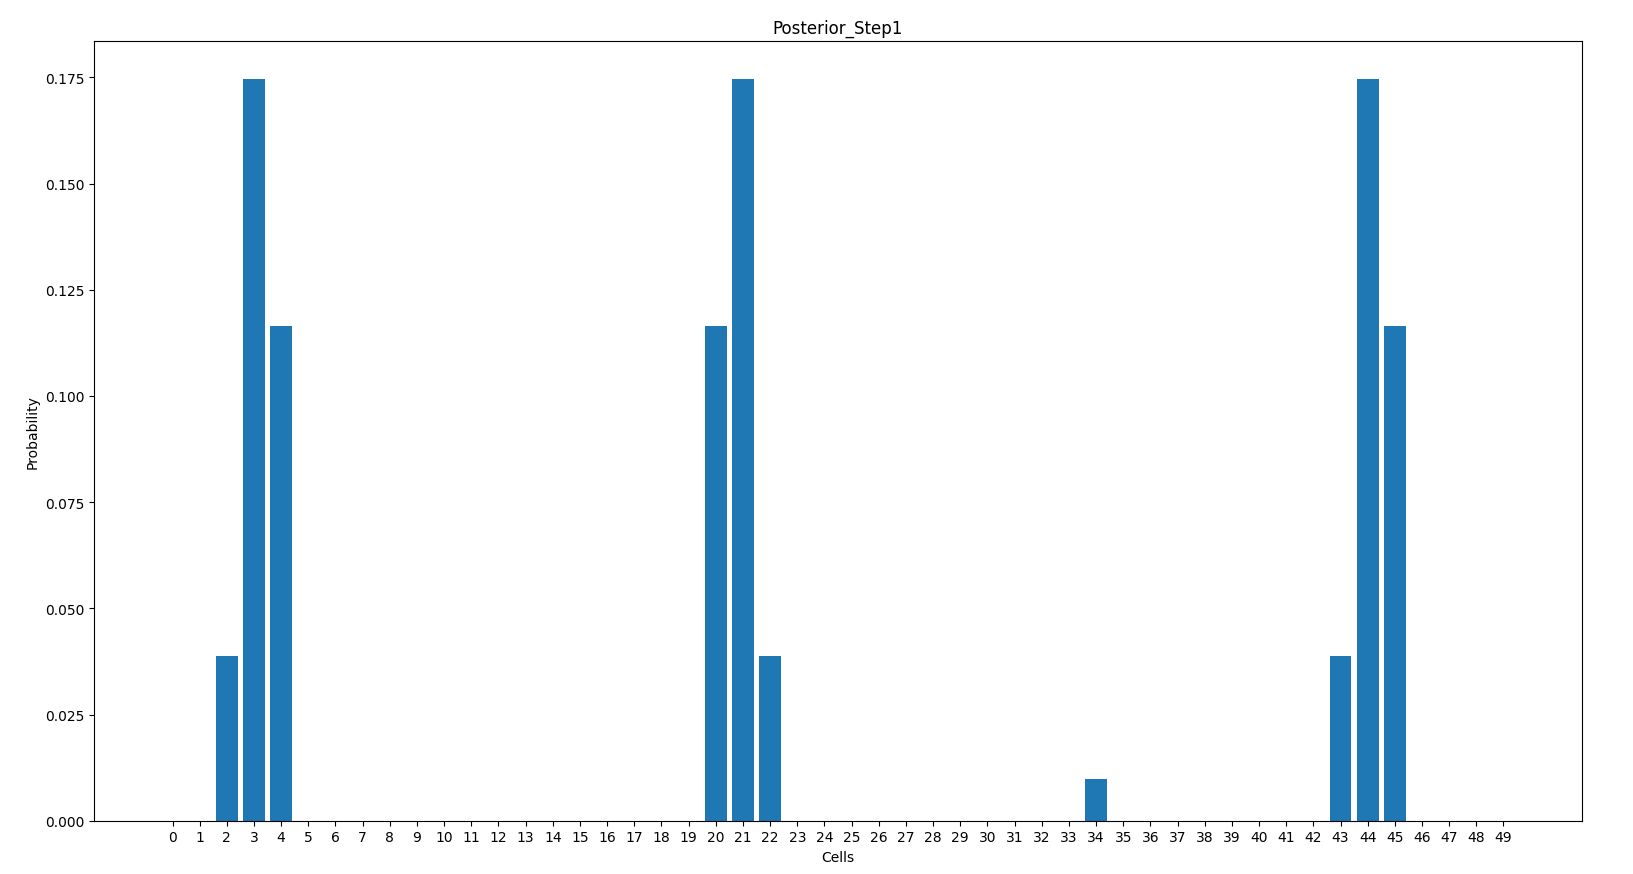
\includegraphics[width=1.3\textwidth]{img/posterior_step_1.png}
    \caption{Posterior Believe nach dem zweitem Schritt=10}
    \label{fig:Posterior Believe nach dem zweitem Schritt=10}
\end{figure}

\begin{figure}[h]
    \centering
    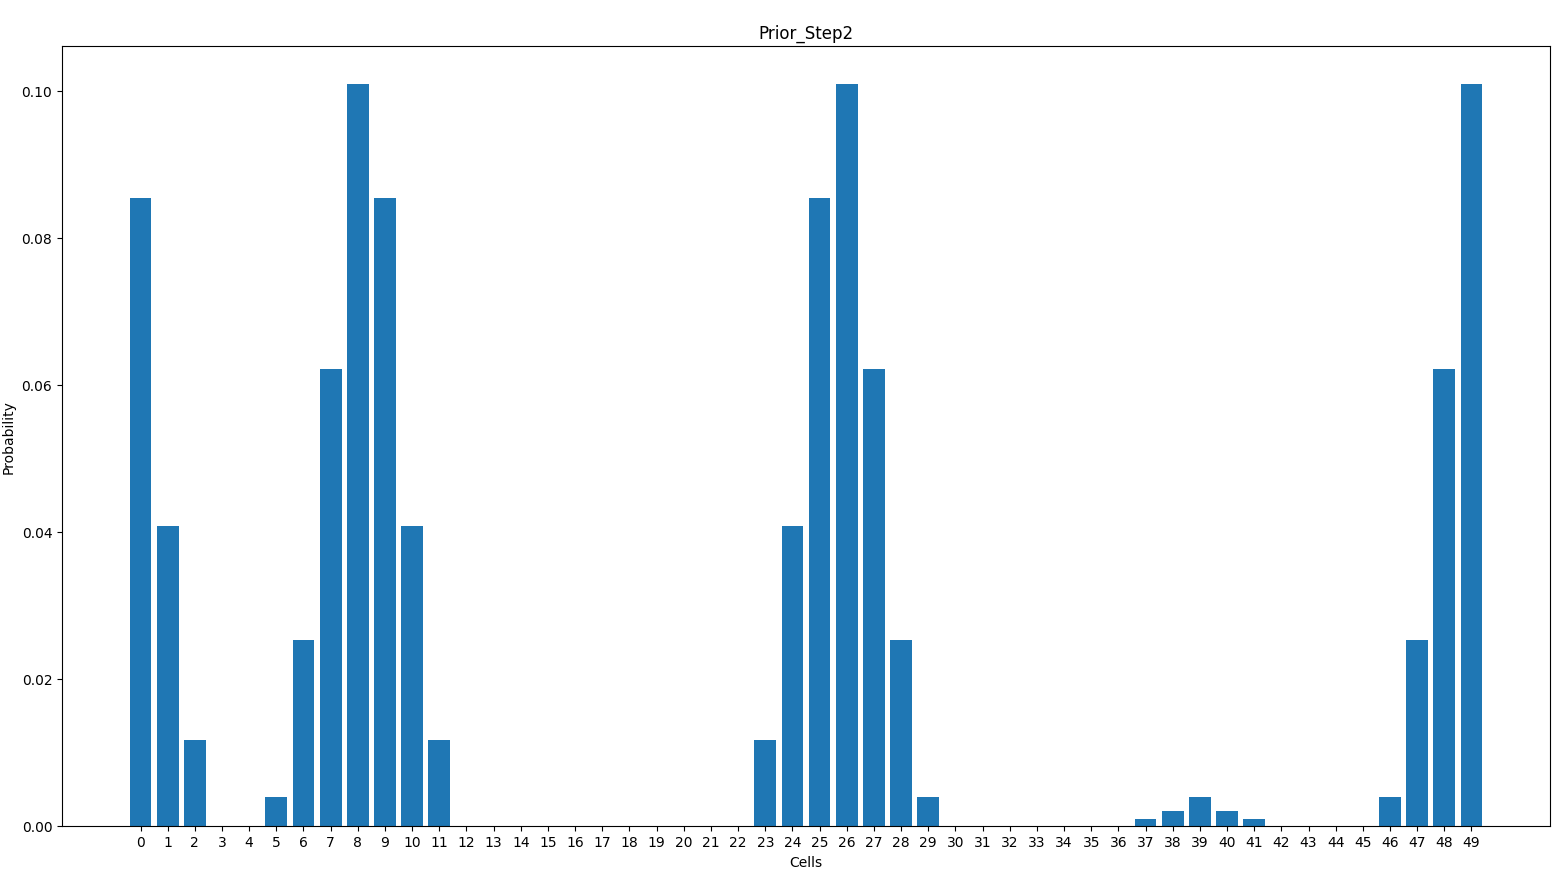
\includegraphics[width=1.3\textwidth]{img/prior_step_2.png}
    \caption{Prior Believe nach dem dritten Schritt=7}
    \label{fig:Initiale Position}
\end{figure}

\begin{figure}[h]
    \centering
    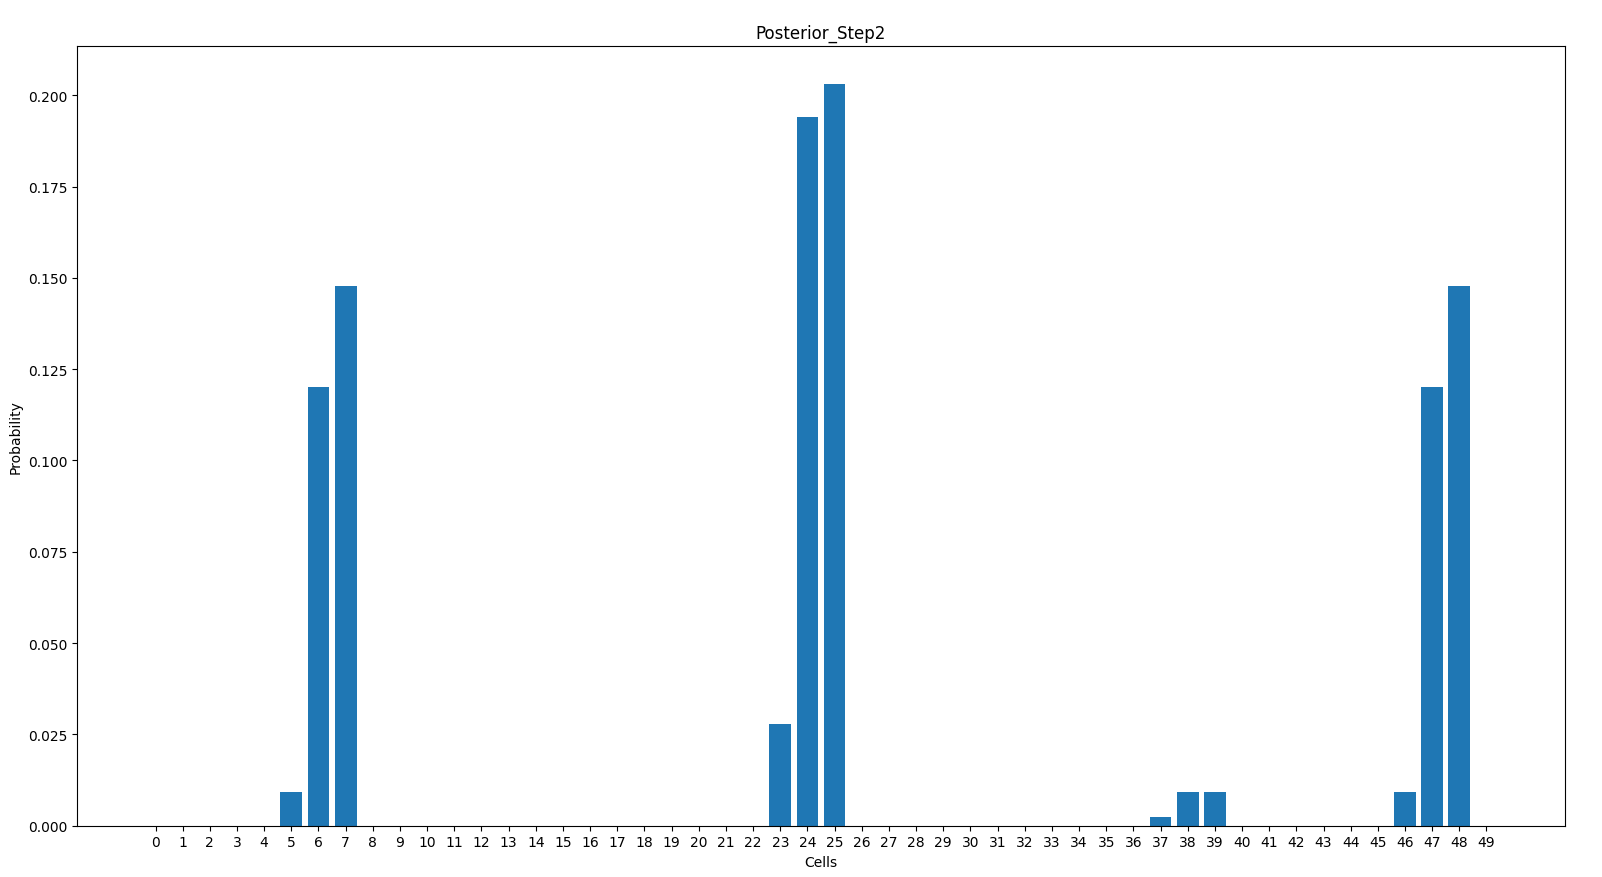
\includegraphics[width=1.3\textwidth]{img/posterior_step_2.png}
    \caption{Posterior Believe nach dem dritten Schritt=7}
    \label{fig:Posterior Believe nach dem dritten Schritt=7}
\end{figure}

\begin{figure}[h]
    \centering
    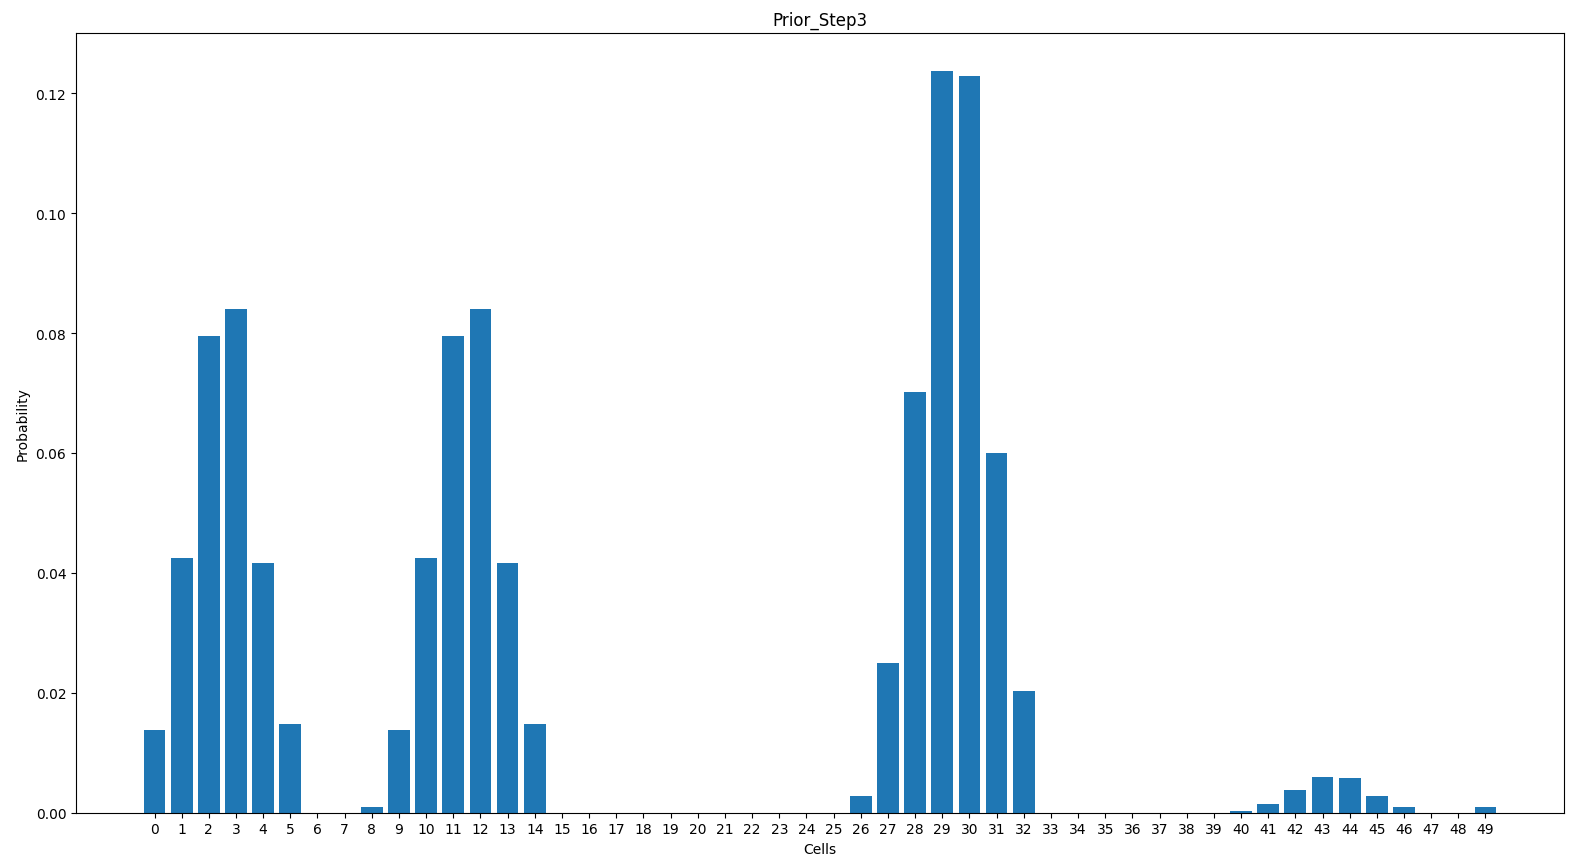
\includegraphics[width=1.3\textwidth]{img/prior_step_3.png}
    \caption{Prior Believe nach dem viertem Schritt=2}
    \label{fig:Prior Believe nach dem viertem Schritt=2}
\end{figure}

\begin{figure}[h]
    \centering
    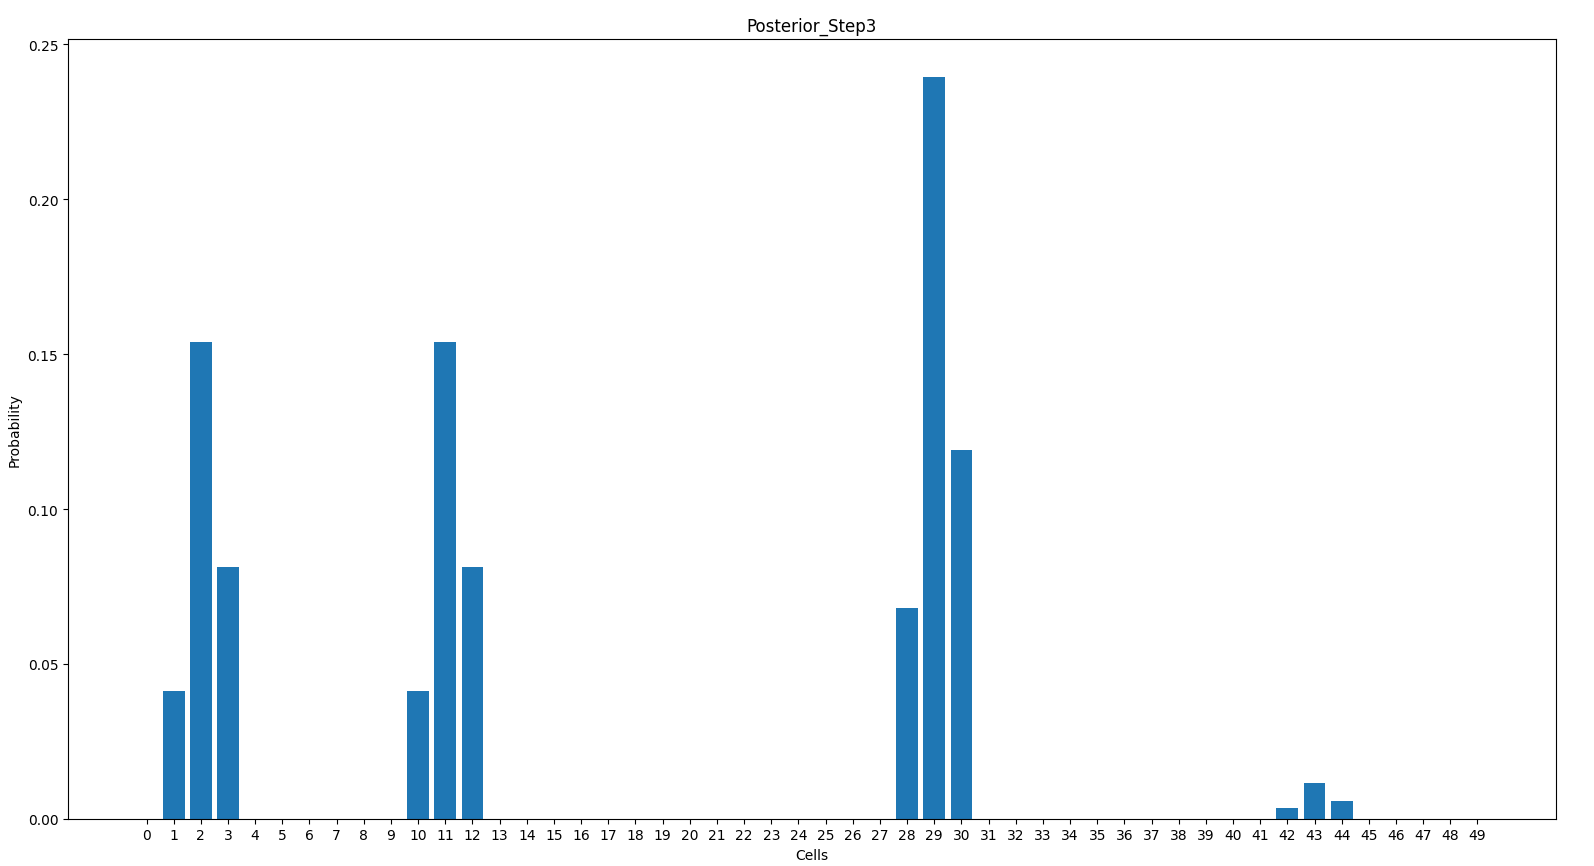
\includegraphics[width=1.3\textwidth]{img/posterior_step_3.png}
    \caption{Posterior Believe nach dem viertem Schritt=2}
    \label{fig:Posterior Believe nach dem viertem Schritt=2}
\end{figure}

\begin{figure}[h]
    \centering
    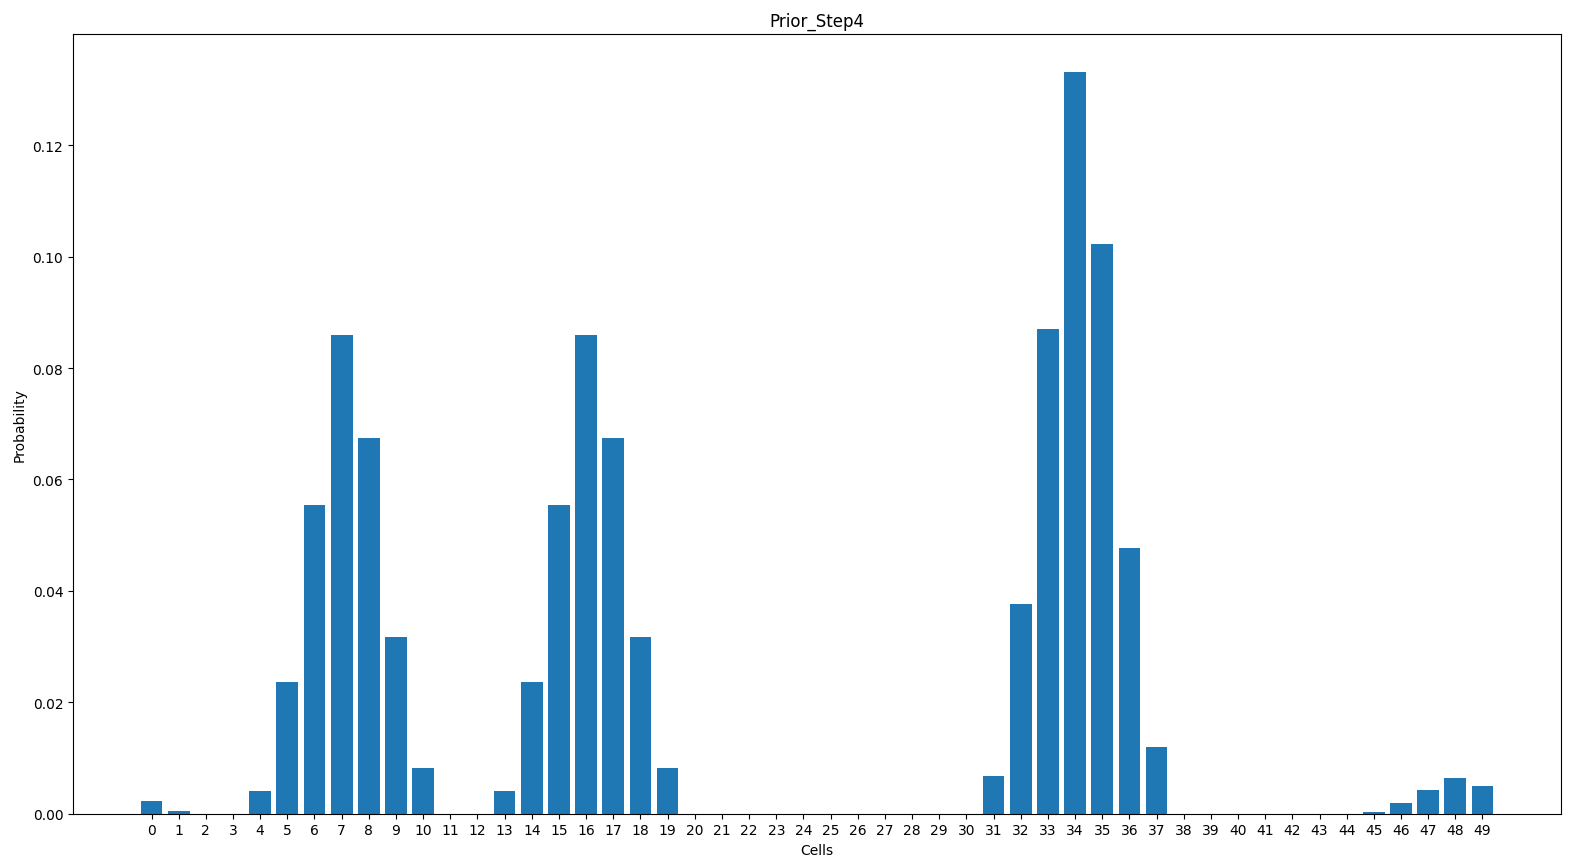
\includegraphics[width=1.3\textwidth]{img/prior_step_4.png}
    \caption{Prior Believe nach dem fünften Schritt=10}
    \label{fig:Prior Believe nach dem fünften Schritt=10}
\end{figure}

\begin{figure}[h]
    \centering
    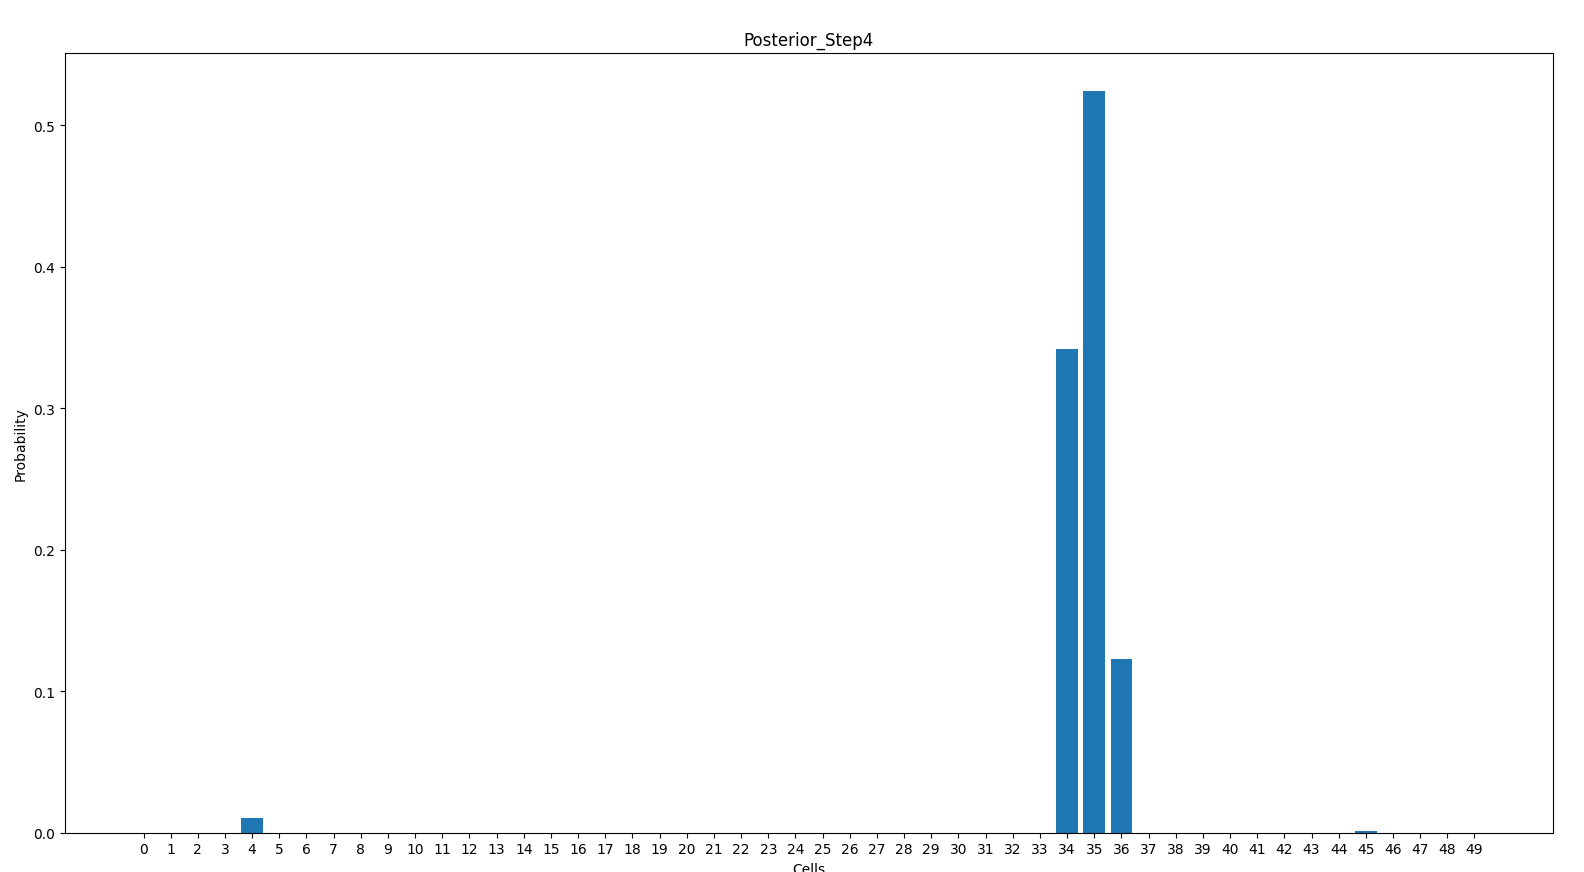
\includegraphics[width=1.3\textwidth]{img/posterior_step_4.png}
    \caption{Posterior Believe nach dem fünften Schritt=10}
    \label{fig:Posterior Believe nach dem fünften Schritt=10}
\end{figure}

\section{Schlussfolgerung}
Wie man sehen kann ist nach dem 5 Schritt die Wahrscheinlichkeit, dass sich der Roboter auf der Zelle 35 mit etwas über 50\% am höchsten. Zusätzlich ist auch erkennbar, dass mit der Erhöhung der Schrittanzahl auch die Genauigkeit sich erhöht.

\end{document}
